\begin{frame}{\large Measuring Reproducibility in Computer Systems Research}

  \begin{figure}
    \centering
    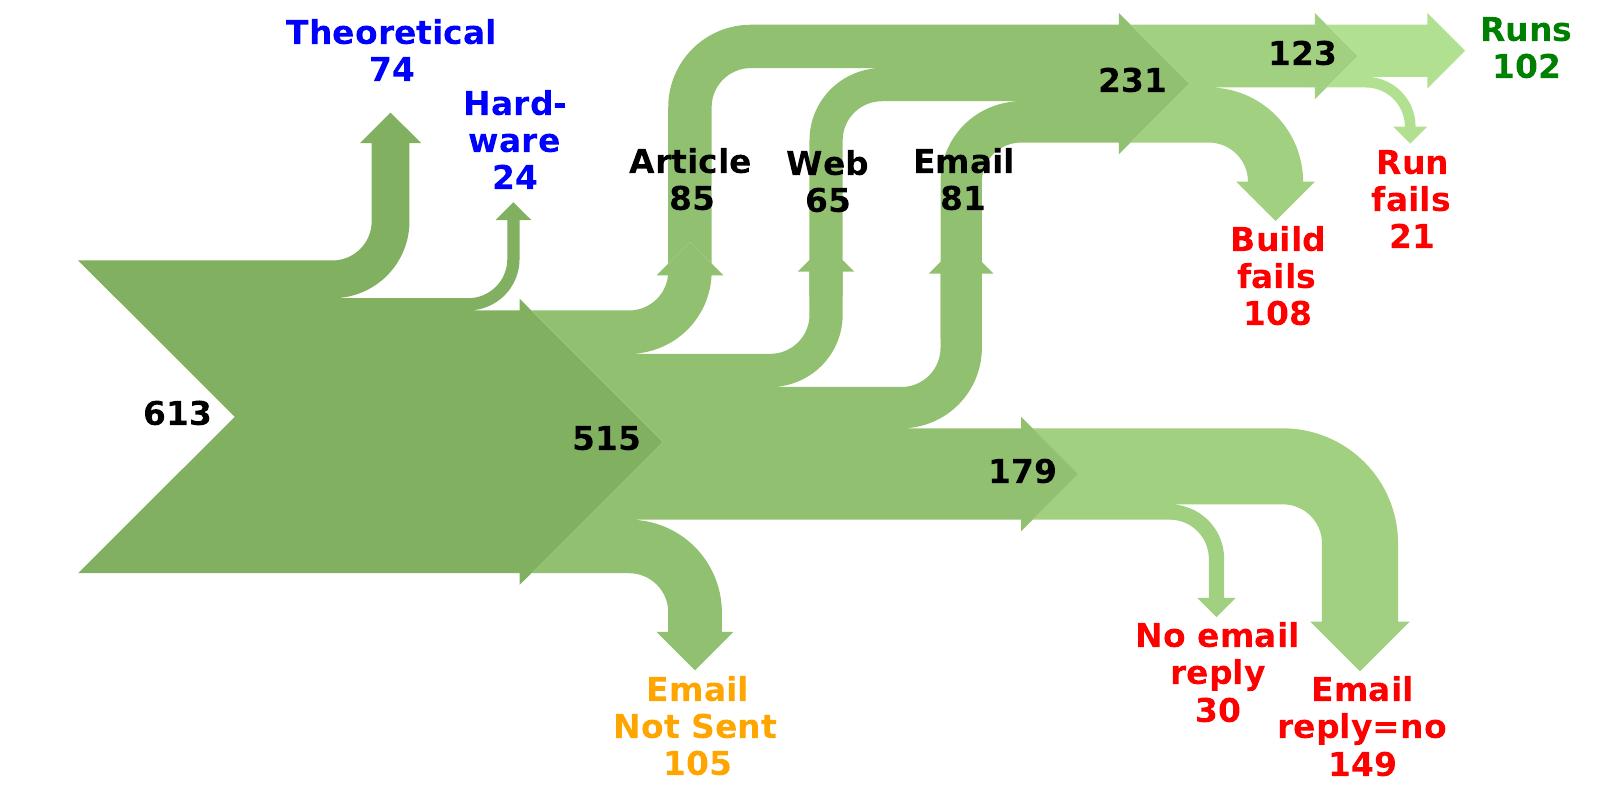
\includegraphics[width=\textwidth]{%
    img/collberg2013_results3.png} %
  \end{figure}
  

  \source{\cite{Collberg2013}}

  \pnote{
    
    613 papers from \\
    - 8 conferences \\
    - 5 journals

    30 minutes of programmer time to try \\
    make build compile/run
    
    Orange: Don't send more than one email to any author \\
    (if author had multiple publications)

    Even if build runs does not even try verify results! \\
    How many more papers will fall off?
    
  }
  
  
\end{frame}

\begin{frame}{}

  \vspace{-0.5cm}
  
  \begin{figure}
    \centering
    
\includegraphics[height=0.785\textheight]{%
    img/benureau2018_cover2.png} %
  \end{figure}
  

  \source{\cite{Benureau2018}}  
  
  
\end{frame}





\begin{frame}{Five \textit{Rs} for scientific code}

  
  \begin{itemize}[leftmargin=2.6cm]
    \itemsep11pt
    \item[$\mathbf{R^1}$ \textit{Re-runnable}:] can be run again when needed (e.g.~more than the one time that was needed to produce the results)

    \item[$\mathbf{R^2}$ \textit{Repeatable}:] program is deterministic, produces repeatable output

    \item[$\mathbf{R^3}$ \textit{Reproducible}:] another researcher can take code \& input data, execute code, and re-obtain same results

    \item[$\mathbf{R^4}$ \textit{Reusable}:] program  can be easily used, and
modified, by you and other people, inside \& outside own lab

    \item[$\mathbf{R^5}$ \textit{Replicable}:] program can be re-implemented by another research to re-obtain results

  \end{itemize}

  

  
  \source{\cite{Benureau2018}}
  
  
\end{frame}



\begin{frame}{$R^0$ -- runnable code}

  \begin{figure}
    \centering
    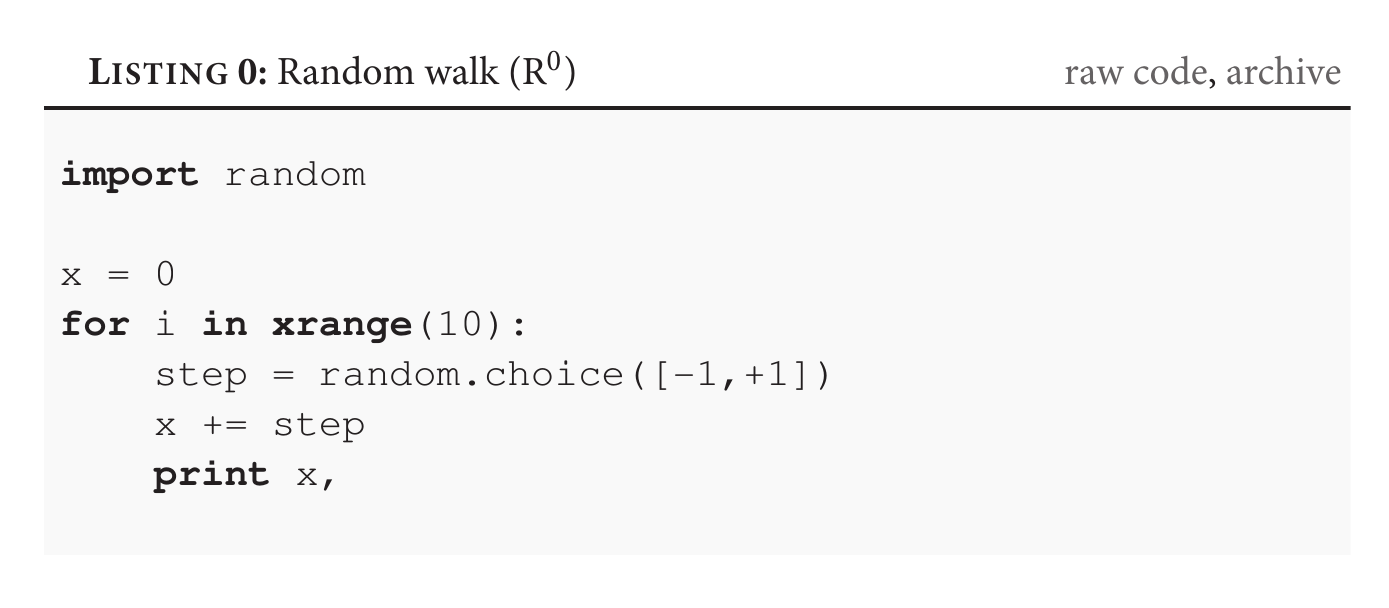
\includegraphics[width=\textwidth]{%
      img/R0_code.png} %
  \end{figure}

  \begin{figure}
    \centering
    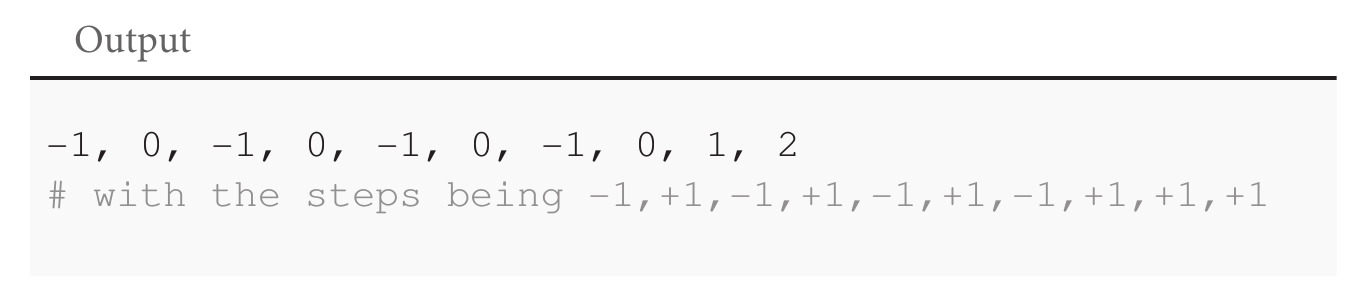
\includegraphics[width=\textwidth]{%
      img/R0_output.png} %
  \end{figure}

  \vspace{1.5cm}  

  \source{\cite{Benureau2018}}
  
  
\end{frame}



\begin{frame}{$R^1$ -- Re-runnable}

  \begin{figure}
    \centering
    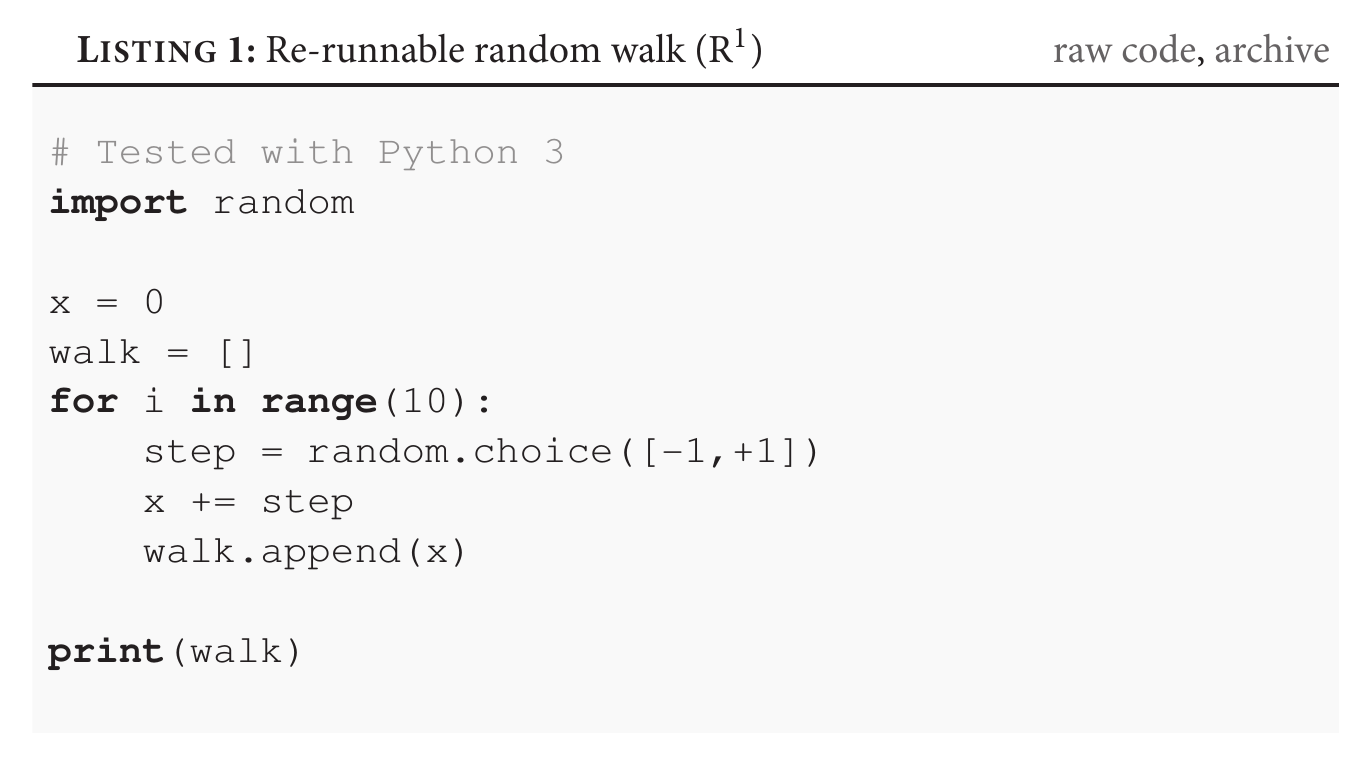
\includegraphics[width=\textwidth]{%
      img/R1_code.png} %
  \end{figure} 
  
  
\end{frame}

\begin{frame}{$R^2$ -- Repeatable}
  
  
  
\end{frame}



\begin{frame}{$R^3$ -- Reproducible}

  \begin{figure}
    \centering
    \includegraphics<1>[width=.8\textwidth]{%
      img/R3_code01.png} %
    \includegraphics<2>[width=.8\textwidth]{%
      img/R3_code02.png} %   
  \end{figure}

  \source{\only<1>{1}\only<2>{2}/2}
    
\end{frame}


\begin{frame}{$R^4$ -- Reusable}

  \begin{figure}
    \centering
    \includegraphics<1>[width=.8\textwidth]{%
      img/R4_code01.png} %
    \includegraphics<2>[width=.8\textwidth]{%
      img/R4_code02.png} %
    \includegraphics<3>[width=.8\textwidth]{%
      img/R4_code03.png} %   
  \end{figure}

    \source{\only<1>{1}\only<2>{2}\only<3>{3}/3}
    
\end{frame}


\begin{frame}{$R^5$ -- Replicable}

  \begin{figure}
    \centering
    \includegraphics<1>[width=.8\textwidth]{%
      img/R5_code01.png} %
    \includegraphics<2>[width=.8\textwidth]{%
      img/R5_code02.png} %   
  \end{figure}

  \source{\only<1>{1}\only<2>{2}/2}
    
\end{frame}
